\documentclass[conference]{IEEEtran}
\usepackage[T1]{fontenc}
\usepackage{cite}
\usepackage{amsmath,amssymb}
\usepackage{booktabs}
\usepackage{url}
\usepackage[hidelinks]{hyperref}
\hypersetup{pdftitle={Estimating Reclaim Benefit Across Cgroups Sharing Compressed Swap},pdfauthor={Adithya Sushil},pdfsubject={Initial research draft, 21 October 2026},pdfkeywords={Linux,zram,cgroups,memory reclaim}}
\usepackage{pgfplots}
\pgfplotsset{compat=1.18}
\newcommand{\MiB}{\,\mathrm{MiB}}
\newcommand{\GiB}{\,\mathrm{GiB}}
\title{Estimating Reclaim Benefit Across Cgroups Sharing Compressed Swap}
\author{\IEEEauthorblockN{Adithya Sushil}
\IEEEauthorblockA{Vellore Institute of Technology\\
Student ID: 24BCI0286\\
\texttt{adithya.sushil2024@vitstudent.ac.in}}}
\begin{document}
\maketitle
\begin{abstract}
Compressed swap can create memory headroom by storing anonymous pages in less
physical memory. Its lasting value depends on the source workload: reclaim may
save little space for poorly compressible pages, and later reuse can erase an
initial saving. We investigate whether a small user-space estimator can measure
the delayed marginal headroom benefit of reclaiming from individual cgroups
sharing one zram device. We implement controlled workloads, a scheduled request
service, an asynchronous reclaim actuator, timestamped telemetry, and a runner
that resets the guest between independent trials. The experimental target is
mean guest headroom during the 20 seconds following a fixed 32-MiB request,
estimated against matched no-action trials. The initial characterization includes 72 trials in 24 complete matched seed blocks. R1 yielded a mean donor-benefit contrast of 28.96 MiB. R2 yielded a mean donor-benefit contrast of 21.34 MiB. R3 yielded a mean donor-benefit contrast of 24.98 MiB.
A separate held-out attribution study supplies 72 usable trials. Its attribution error under unrelated memory activity prevents advancement to coordinated-policy evaluation. These observations characterize the measurement problem. Held-out
future-action prediction, coordinated-policy evaluation, and comparisons with
active Senpai and feedback-equipped DAMOS remain necessary before a controller
improvement can be claimed.
\end{abstract}
\begin{IEEEkeywords}
Linux, memory reclamation, compressed swap, zram, cgroups, experimental systems
\end{IEEEkeywords}

\section{Introduction}
An operating system can reclaim memory from background applications while
preserving the responsiveness of a foreground service. When the swap backend is
zram, reclaimed pages remain in RAM in compressed form. Their logical size and
their physical allocator footprint can differ substantially~\cite{zram}. The
benefit of selecting a particular source application also depends on when the
evicted contents are needed again.

Consider two programs with the same resident allocation and hot-region size.
One may contain easily compressible data but promptly revisit reclaimed pages;
another may leave its reclaimed contents unused for the next several seconds.
A controller should account for this delayed behavior when deciding where to
spend its next unit of reclaim work. An immediate resident-memory decrease alone
does not answer that question.

The research hypothesis is that historical, serialized probes can provide
useful estimates of delayed marginal guest-headroom benefit, and that these
estimates can improve donor selection under one shared reclaim-work budget.
This hypothesis has three separable requirements: donor choice must produce a
repeatable effect; an estimator must generalize to unseen decisions; and the
resulting policy must improve a useful resource tradeoff. A successful
characterization establishes only the first requirement.

The present contribution is an implemented measurement artifact and an initial
characterization of fixed-dose source selection. The artifact preserves failed
attempts, verifies application results, includes generator queueing in latency,
and records actual actuator cost. The broader estimator and allocator remain
candidates whose value requires the later experiments described here.

\section{Background and Related Work}
Linux cgroup v2 supplies per-group memory accounting and a proactive
\texttt{memory.reclaim} interface. The requested amount is a control input:
the kernel may reclaim more or less, and a request can return
\texttt{EAGAIN} after partial effects~\cite{cgroup}. Pressure Stall Information
(PSI) quantifies time lost to resource contention~\cite{psi}. These interfaces
enable observation and intervention without a custom reclaim mechanism.

TMO and its Senpai controller already use application sensitivity and delayed
pressure feedback to adjust offloading~\cite{tmo}. DAMON-based operation schemes
(DAMOS) support access-aware actions, quotas, filters, and externally supplied
goals~\cite{damon}. Consequently, feedback, work limits, and foreground
protection are established ingredients. A fair eventual comparison must supply
existing systems with comparable application feedback and verify that their
configured mechanisms actually perform reclaim.

The controlled study by Dhakal and Sigdel~\cite{bounded} is particularly close
to the pilot setting: it evaluates a one-time bounded cgroup reclaim request
with compressed swap and checked foreground workloads. Our initial study
varies the source donor and estimates delayed headroom effects using matched
controls. Repeating an actuator loop or reproducing an ARM VM environment alone
would not establish an additional systems contribution.

Acclaim already addresses foreground-aware eviction and predictive background
reclaim~\cite{acclaim}; Ariadne uses hotness-aware organization and adaptive
compression for mobile relaunch~\cite{ariadne}. Later reuse and compression cost
are therefore established considerations rather than new observations here.

App-aware swapping also has substantial overlap. appSwap uses application
behavior and reuse information when managing swap resources~\cite{appswap}.
ZramPool investigates adaptive zram-instance management~\cite{zrampool}. Our
candidate concerns intervention-estimated benefit when selecting source cgroups
under one proactive-work budget. The inspected public ZramPool artifact
predates its final journal version~\cite{zrampoolcode}; the final full text
remains an unresolved overlap check. We make no universal novelty or
superiority claim about either system.

\section{Problem Definition}
Let $H(t)$ denote the guest's \texttt{MemAvailable}, and let $q$ be a reclaim
request issued to donor $i$ at time $t_0$. The target is
\begin{equation}
G_i(q,T)=\mathbb{E}\!\left[\frac{1}{T}\int_{t_0}^{t_0+T}
\left(H_i^{(q)}(t)-H^{(0)}(t)\right)dt\right],
\label{eq:target}
\end{equation}
where $H^{(0)}$ is the potential headroom trajectory without that intervention.
Only one trajectory is observed in a trial. We approximate the contrast with
separate randomized, matched action and no-action trials:
\begin{equation}
\widetilde{G}_i =
(\bar H_{i,\mathrm{post}}-\bar H_{i,\mathrm{pre}})
-(\bar H_{0,\mathrm{post}}-\bar H_{0,\mathrm{pre}}).
\label{eq:reference}
\end{equation}
The reference is noisy and does not measure exact donor ownership of physical
zram allocator pages. \texttt{MemAvailable} already reflects RAM consumed by
zram; subtracting the allocator footprint again would double-count that cost.
Allocator, residency, swap, and refault counters provide supporting diagnostics.

The horizon begins at request dispatch, so a slow actuator consumes part of the
evaluation window. Latency, useful background progress, and measured reclaim
wall/CPU time are separate outcomes. Requested bytes are never substituted for
observed memory benefit. Guest headroom is the scope of the claim; RAM returned
by the hypervisor to the macOS host is a separate outcome.

\section{Artifact and Candidate Controller}
\subsection{Workloads and Measurement Path}
The artifact uses C for the donor, request service, and reclaim worker, and
Python's standard library for orchestration and analysis primitives. Each donor
allocates and touches private anonymous pages. Structured data repeat a
non-uniform 64-byte motif within each page; the alternative uses seeded
pseudorandom words. Donors read a hot region while performing a fixed arithmetic
operation sequence and reporting completed work units. A checksum before and
after execution verifies memory integrity. Verification after the measurement
does not contribute to the reported foreground or headroom windows.

The foreground service has a 128-MiB working set. Requests carry an identifier
and key, and replies contain an independently checked deterministic result.
The client schedules arrivals independently of earlier completions. Latency is
completion time minus scheduled arrival; failed, incorrect, and missed requests
are retained. The client bounds outstanding work, and generator lateness remains
observable. Repeated keys are used to precompute expected results before timing.

The collector polls every 250 ms, retaining original interface text and parsed
values. Each scan has start/end timestamps because reading multiple files is
not atomic. Optional fields remain missing when unavailable. A separate process
issues reclaim, so a slow kernel call cannot block collection. The worker accepts
only registered donor IDs and bounded page-aligned requests, rejects duplicate
IDs, and records dispatch, completion, wall time, CPU time, and errno.

\subsection{Estimation and Shared Work Admission}
The implemented E1 candidate stores the latest isolated delayed probe effect.
Before a probe, it fits a linear drift estimate $\hat s$ to a quiet history
window; after the observation horizon, it computes
\begin{equation}
\widehat{G}^{\mathrm{probe}}_i=
\bar H_{\mathrm{post}}-\bar H_{\mathrm{pre}}-\hat sT.
\end{equation}
An uncertainty penalty grows as the evidence ages. Missing, stale, or flagged
evidence produces an explicit UNKNOWN result. The current uncertainty envelope
is a heuristic derived from quiet-window residual variation and a floor; it is
not a calibrated confidence interval. A post-probe estimate is evidence for a
later decision, not a prediction made before the measured probe.

The candidate policy can rank eligible donors by a conservative delayed-benefit
estimate divided by estimated action cost, with a positive cost floor. Initial
probes and later re-probes share one ledger. The initial admission cap is eight
32-MiB requests, with a separately configured accumulated actuator-wall-time
cap. One action is in flight globally, and actions are spaced to observe delayed
effects. Calls can exceed the remaining admission-time allowance; overshoot is
recorded and prevents subsequent dispatch. This is not a hard kernel-CPU bound.

Policies for no proactive action, round-robin, observable coldness, immediate
gain, and delayed benefit are implemented. Their execution is gated on recorded
characterization and held-out estimator checks. The characterization reported
here does not evaluate these policies. Foreground latency and donor progress
thresholds must be calibrated and frozen before a policy experiment.

\section{Experimental Method}
\subsection{Environment and Calibration}
Experiments run in a dedicated Debian 13 ARM64 guest on an Apple Silicon Mac
with 16 GiB of host RAM. The guest has 3 GiB RAM, two vCPUs, a 40-GiB provisioned
virtual disk, and kernel \texttt{6.12.113+deb13-arm64}. It is launched through
Apple Virtualization.framework. This is a recorded deviation from the plan's
UTM launcher; all comparisons use the same backend. The official Debian cloud
image's SHA-512 digest was checked against the downloaded checksum list.

The only active swap backend is a 1-GiB logical zram device using lz4. zswap and
zram writeback are disabled, and guest swappiness is 100. The initialized swap
header occupies one zram page even when logical swap usage is zero. Every
independent trial starts after a guest reboot, checks the starting store state,
and records a fresh kernel boot ID. Each worker enters its cgroup before the
large allocation. Containment settings are identical across arms.

An unpressured sequential-client calibration with 65,536 memory touches per
request completed 1,000 requests in 0.501 s, approximately 1,996 requests/s.
This includes connection and client overhead and is not a proven service
maximum. The initial characterization freezes 200 scheduled requests/s to keep
the client and observation path stable and provide approximately 4,000 requests
per 20-s window. This load is about 10\% of that capacity estimate; later policy
studies must examine higher offered loads as well.

The first calibration with a hot prefix showed rapid swap-in and loss of the
initial saving. A separately logged calibration moved the initial hot region to the
mapping's high-address end, leaving a cold prefix. The two calibration attempts
are retained and excluded from discovery blocks. All discovery arms use the
same frozen layout. This workload construction is a validity limitation to test
with other allocation/access orders.

\subsection{Randomized Fixed-Dose Characterization}
Each discovery block contains three fresh trials: no proactive action, one
32-MiB request to A, and one to B. Arm order is randomized within a seed block;
block order is also randomized. The frozen matrix contains eight independent
blocks in each of three regimes, for 72 discovery trials. A trial has 5 s of
warm-up, 20 s before dispatch, a 20-s delayed horizon, and 5 s of recovery
observation. Each donor initially allocates 512 MiB. These are proactive
characterization workloads; successful headroom recovery alone does not
establish behavior under severe memory pressure.

\begin{table}[t]
\caption{Prespecified Donor Regimes}
\label{tab:regimes}
\centering\small
\begin{tabular}{@{}p{.07\columnwidth}p{.84\columnwidth}@{}}
\toprule
ID & Controlled distinction \\
\midrule
R1 & Equal footprint/hot fraction with structured versus random contents. A/B data identities alternate across blocks. \\
R2 & Equal contents and work rate; one donor expands reuse from 32 to 512 MiB one second after dispatch. \\
R3 & Compressibility contrast plus an unrelated 192-MiB resident allocation from 4 to 14 s after dispatch. \\
\bottomrule
\end{tabular}
\end{table}

R2 isolates delayed reuse without rewriting page contents. R3 is a controlled
resident-memory interference case; it does not by itself cover every form of
shared compressed-pool interference. Workload identities, content labels,
future phases, matched control outcomes, and held-out reference gains are
evaluation metadata and must not enter an online policy.

\subsection{Analysis and Advancement Criteria}
Headroom means use time-weighted trapezoidal integration with interpolated
window boundaries and no extrapolation. The prespecified donor contrast is the
structured minus random donor in R1/R3 and the non-reusing minus reusing donor
in R2. The no-action arm estimates baseline drift for each donor effect; it
cancels from the A-versus-B difference within a block. We resample independent
seed blocks for 95\% bootstrap intervals. Individual service requests are not
treated as independent experimental replicates.

The practical Checkpoint A requires a repeatable donor distinction, with an
initial target of 8 MiB for the fixed 32-MiB request. The artifact additionally
checks at least eight complete blocks and a positive contrast interval in R1/R2.
These are project advancement criteria, not general statistical standards.
Timeout, OOM, and performance harm are adverse outcomes. Predeclared technical
invalidity includes a failed measurement path, incomparable reset, or overloaded
generator; such attempts remain in the execution record.

\section{Initial Results}
This draft analyzes 72 trials belonging to 24 complete matched seed blocks. The execution log contains 72 selected attempts, 0 failed attempts, 0 technically invalid attempts, and 0 attempts with recorded adverse outcomes. Incomplete blocks remain visible in the artifact and are omitted only from paired contrasts requiring all three arms.

In R1, the mean prespecified donor contrast was 28.96 MiB (95\% block-bootstrap interval [16.76, 43.34]). In R2, the mean prespecified donor contrast was 21.34 MiB (95\% block-bootstrap interval [15.50, 27.70]). In R3, the mean prespecified donor contrast was 24.98 MiB (95\% block-bootstrap interval [19.01, 31.93]).

\begin{table}[t]
\caption{Delayed Donor-Benefit Contrast, in MiB}
\label{tab:results}
\centering\small
\begin{tabular}{@{}lrrl@{}}
\toprule
Regime & Blocks & Mean gap & 95\% interval \\
\midrule
R1 & 8 & 28.96 & [16.76, 43.34] \\
R2 & 8 & 21.34 & [15.50, 27.70] \\
R3 & 8 & 24.98 & [19.01, 31.93] \\
\bottomrule
\end{tabular}
\end{table}

The prespecified practical Checkpoint A was met for the compressibility and delayed-reuse regimes. This authorizes estimator validation; it does not establish the proposed policy's value.
Observed before/after changes from the two calibration attempts are not used
as matched causal estimates. Successful actuator return values likewise do
not establish reclaimed physical bytes. Application checksums and saved
request logs support functional correctness, while measured errors, cost, and
adverse outcomes remain part of the resource tradeoff.

\begin{figure}[t]
\centering
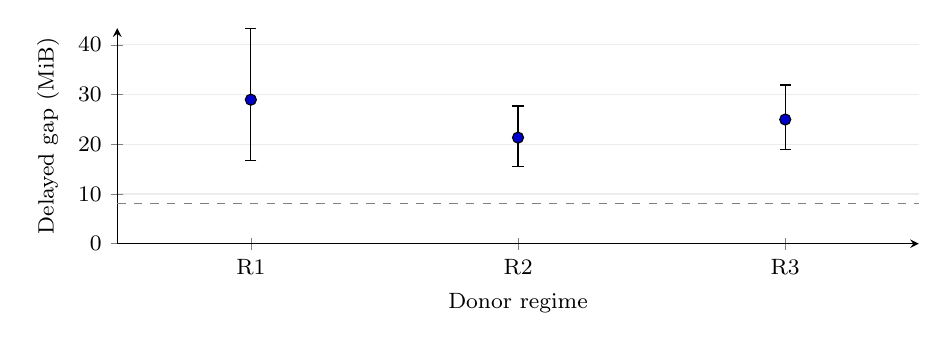
\begin{tikzpicture}
\begin{axis}[width=.97\columnwidth,height=1.7in,
  xlabel={Donor regime},ylabel={Delayed gap (MiB)},
  tick label style={font=\footnotesize},label style={font=\footnotesize},
  xtick={1,2,3},xticklabels={R1,R2,R3},
  xmin=.5,xmax=3.5,ymin=0,axis lines=left,ymajorgrids=true,grid style={gray!15}]
\addplot+[only marks,mark=*,black,error bars/.cd,y dir=both,y explicit]
table[x=x,y=mean,y error minus=lo,y error plus=hi] {
x mean lo hi
1 28.964422 12.209040 14.374484
2 21.336823 5.833591 6.364584
3 24.979767 5.972887 6.946096
};
\addplot[gray,dashed,domain=.5:3.5] {8};
\end{axis}
\end{tikzpicture}
\caption{Prespecified delayed donor contrast with 95\% seed-block bootstrap
intervals. The dashed line marks the initial 8-MiB practical target.}
\label{fig:gaps}
\end{figure}
An exploratory sensitivity analysis reuses the same discovery blocks at 2, 5, 10, 20, and 24 s. In R2, the mean donor contrast is 2.56 MiB at 2 s (95\% interval [-3.43, 8.93]) and 21.34 MiB at the primary 20-s endpoint. The paired 20-s-minus-2-s difference is 18.77 MiB ([17.88, 19.65]). These correlated horizons do not supply additional independent replicates or replace the prespecified endpoint. Their intervals are descriptive and are not multiplicity-adjusted. The full sensitivity results are preserved in the artifact.

The post-dispatch windows contain 288,000 scheduled foreground arrivals and 0 failed, missed, or incorrect replies. Table~\ref{tab:latency} reports the mean of independent-run p99 values. These reference arms do not establish a calibrated service-protection guarantee.

\begin{table}[t]
\caption{Mean Run-Level Foreground p99, in Milliseconds}
\label{tab:latency}
\centering\small
\begin{tabular}{@{}lrrr@{}}
\toprule
Regime & No action & Reclaim A & Reclaim B \\
\midrule
R1 & 3.78 & 3.80 & 3.90 \\
R2 & 4.31 & 4.01 & 4.22 \\
R3 & 3.98 & 3.95 & 3.94 \\
\bottomrule
\end{tabular}
\end{table}
\subsection{Held-Out Post-Probe Attribution}
A separate frozen phase contains 74 held-out reference attempts, yielding 72 usable trials in complete matched blocks, using new seeds, later reuse timings, and different interference allocations. E1 is evaluated after each probe's horizon against matched reference effects; held-out references are never estimator inputs. This evaluates attribution of an observed probe, not advance prediction of that intervention.

\begin{table}[t]
\caption{Held-Out E1 Attribution Diagnostics}
\label{tab:estimator}
\centering\small
\begin{tabular}{@{}lrrr@{}}
\toprule
Regime & MAE (MiB) & Rank (\%) & Envelope (\%) \\
\midrule
R1 & 3.89 & 100.0 & 25.0 \\
R2 & 3.28 & 100.0 & 43.8 \\
R3 & 116.54 & 100.0 & 0.0 \\
\bottomrule
\end{tabular}
\end{table}
MAE is mean absolute attribution error. Ranking uses material donor differences of at least 8 MiB. Envelope coverage is the fraction of reference effects inside E1's heuristic uncertainty envelope; it is not a calibrated confidence level. Errors are resampled by matched seed block. The engineering protocol, frozen before validation, requires useful coverage, at least 80\% ranking accuracy, and either predictable abstention under interference or mean error no greater than the 8-MiB practical resolution with at least 80\% heuristic-envelope coverage.

For R1, the 95\% block-bootstrap MAE interval is [2.87, 4.90] MiB; known-estimate coverage is 100.0\%. There are 8 correct rankings among 8 ranked material pairs (95\% Wilson interval [67.6, 100.0]\%). For R2, the 95\% block-bootstrap MAE interval is [2.31, 4.27] MiB; known-estimate coverage is 100.0\%. There are 8 correct rankings among 8 ranked material pairs (95\% Wilson interval [67.6, 100.0]\%). For R3, the 95\% block-bootstrap MAE interval is [82.41, 152.02] MiB; known-estimate coverage is 100.0\%. There are 8 correct rankings among 8 ranked material pairs (95\% Wilson interval [67.6, 100.0]\%). 

The baseline candidate does not meet Checkpoint B. Its interference bias demonstrates why a useful donor ranking can coexist with an unusable benefit estimate. Unrelated memory activity must be accounted for, or the estimator must abstain reliably. Coordinated-policy evaluation is therefore deferred pending a declared estimator redesign. This finding does not rule out better estimators.

The execution record retains 2 technical-invalid attempts exceeding the predeclared 100-ms generator lateness limit. Only those arms are repeated, with the exact frozen source, settings and seeds; adverse outcomes are not grounds for repetition.

\subsection{Collector Overhead}
A separate validity study uses 8 randomized fresh-boot on/off pairs with the same workloads and a 40-s measurement interval. The collector consumes a mean 454.52 ms of thread CPU per interval (95\% block-bootstrap interval [435.89, 473.86] ms). Incremental harness RSS growth is 7.48 MiB ([7.46, 7.51]); the mean foreground p99 on/off ratio is 1.021 ([0.992, 1.061]). Thread CPU is read from the collector's Linux pthread CPU clock. Matched harness differences include interactions with client logging and scheduling. This validity phase does not tune the frozen estimator.

The observer study uses a dispatcher-only extension recorded as a separate source version. The exact original research runtime is restored for technical repeats. All executed versions are archived; donor, foreground, collector, and estimator implementations are unchanged across these phases.


\section{Remaining Validation and Threats to Validity}
Follow-up estimator experiments must address the observed attribution failure,
freeze revised parameters, and use fresh seeds and access patterns. It should predict a future intervention from
past/present telemetry, then compare that prediction with matched experimental
references. Report MiB error, sign mistakes, donor-ranking accuracy, uncertainty
coverage, abstention coverage, and cost by regime. A target of 80\% ranking
accuracy is meaningful only with confidence intervals and useful coverage.
Scoring an estimate after observing its target intervention does not establish
future-action predictive value.

Only after estimator validation should the five candidate policies be run on
unseen ranking reversals and interference with common eligibility rules and
resource caps. Foreground p99 and donor progress are constraints, and actual
work consumption must be compared alongside permitted caps. If immediate gain
or coldness performs equally well, the added estimator's necessity has not been
established. Later comparisons require active, version-pinned Senpai and DAMOS
with comparable application feedback, a simple measured-gain extension, and a
same-estimator round-robin variant.

The current study uses synthetic anonymous-memory donors, one host, one
compressor, one guest size, and a modest offered load. Its headroom signal is a
kernel estimate affected by unrelated activity. The cold-prefix layout and
deterministic request-key cycle can influence results. A full study must add
allocation-order sensitivity, stronger pressure, file-backed donors, a checked
SQLite service, resource-size variation, other arrival/access patterns, and overhead sensitivity under stronger
pressure. Two VMs on one host do not constitute independent hardware. Host memory
snapshots are retained, while the host CPU-load query was unavailable under
the execution permissions; host interference is not fully controlled. The primary harness CPU counter includes client and orchestration work; the
separate on/off study and thread clock isolate the collector's incremental cost.

No independent reproduction or strong-baseline experiment has yet been
completed. Related-work overlap, including the final ZramPool text, must be
resolved before submission. This manuscript is an initial research draft dated
21 October 2026, not evidence of an accepted or completed systems contribution.

\section{Conclusion}
We implement a reproducible path for measuring delayed headroom effects of
fixed-dose reclaim from cgroups sharing compressed swap. The artifact connects
controlled workloads, scheduled and checked requests, asynchronous intervention,
raw telemetry, and independent randomized trials. The resulting characterization
tests whether source selection is worth learning in this setting. Validated
future-action estimates and useful improvement over strong alternatives remain
the requirements for the proposed controller contribution.

The held-out baseline fails the usefulness and reliability gate. The next mechanism step is a declared estimator redesign that separates intervention benefit from unrelated memory activity, followed by fresh validation.

\section*{Artifact Availability}
The local artifact includes source, guest provisioning, a headless VM launcher,
frozen configurations, every attempted run, analysis scripts, and this standalone
IEEEtran source. The guest image and tool downloads are excluded from the source
archive; their provenance is recorded separately. No public artifact URL is
claimed in this draft.

\begin{thebibliography}{11}
\bibitem{zram} The Linux Kernel Community, ``zram: Compressed RAM-based block devices,'' Linux v6.12 documentation. [Online]. Available: \url{https://www.kernel.org/doc/html/v6.12/admin-guide/blockdev/zram.html}
\bibitem{cgroup} T. Heo, ``Control Group v2,'' Linux kernel documentation. [Online]. Available: \url{https://docs.kernel.org/admin-guide/cgroup-v2.html}
\bibitem{psi} J. Weiner, ``PSI---Pressure Stall Information,'' Linux kernel documentation. [Online]. Available: \url{https://docs.kernel.org/accounting/psi.html}
\bibitem{tmo} J. Weiner \emph{et al.}, ``TMO: Transparent Memory Offloading in Datacenters,'' in \emph{Proc. ASPLOS}, 2022, pp. 609--621, doi: 10.1145/3503222.3507731.
\bibitem{damon} The Linux Kernel Community, ``DAMON: Design,'' Linux v6.12 documentation. [Online]. Available: \url{https://www.kernel.org/doc/html/v6.12/mm/damon/design.html}
\bibitem{bounded} A. Dhakal and S. Sigdel, ``A Bounded Reclaim Actuator for PSI-Guided Compressed Memory: A Controlled Ablation,'' arXiv:2608.13689v1, Aug. 2026. [Online]. Available: \url{https://arxiv.org/abs/2608.13689}
\bibitem{acclaim} Y. Liang \emph{et al.}, ``Acclaim: Adaptive Memory Reclaim to Improve User Experience in Android Systems,'' in \emph{Proc. USENIX ATC}, 2020, pp. 897--910.
\bibitem{ariadne} Y. Liang \emph{et al.}, ``Ariadne: A Hotness-Aware and Size-Adaptive Compressed Swap Technique for Fast Application Relaunch and Reduced CPU Usage on Mobile Devices,'' arXiv:2502.12826, Feb. 2025.
\bibitem{appswap} Y.-C. Wei, Y.-C. Tsou, Y.-C. Chen, and L.-P. Chang, ``App-aware Swap Resource Allocation for Enhancing User-perceived Latency on Mobile Devices,'' \emph{ACM Trans. Embedded Comput. Syst.}, vol. 24, no. 5s, pp. 1--24, 2025, doi: 10.1145/3760385.
\bibitem{zrampool} Y. Deng, G. Xie, C. Xiong, S. Zhao, W. Ren, and K. Li, ``Zram Instance Pool Framework for Adaptive Memory Compression in Resource-Sensitive Embedded Operating Systems,'' \emph{IEEE Trans. Comput.-Aided Design Integr. Circuits Syst.}, vol. 44, no. 8, pp. 2925--2938, 2025, doi: 10.1109/TCAD.2025.3533300.
\bibitem{zrampoolcode} ESNL-HNU, ``ZramPool public source artifact,'' commit cda6562a11b7ca4ca82098a3505f8f11d707baf9, May 2023. [Online]. Available: \url{https://github.com/esnl-hnu/zrampool}
\end{thebibliography}
\end{document}
